\section{ResUNet-a}
\label{sec:Chapter25}

ResUNet-a je bohaté rozšířeni původní sítě U-Net o hned několik změn, poprvé představeno v literatuře \cite{resuneta} roku 2019. Síť je obohacena o \textbf{reziduální bloky} (představeny v \cite{residualblocks}), \textbf{dilatované konvoluce}, \textbf{PSP pooling} (představeny v \cite{psp}) vrstvy a \textbf{multi-taskové učení}. Síť je také v této literatuře trénována na své adaptaci Diceovy loss funkce. Vysoko-úrovňová podoba sítě je představena na obrázku \ref{fig:resuneta_overview}.

\textbf{Reziduální bloky} jsou zde použity namísto klasických bloků U-Net jak v enkodéru, tak v dekodéru původní architektury U-Net. Slouží pro adresování problému explodujících či ztrácejících se gradientů při fázi učení hlubokých sítí. Do reziduálních bloků jsou také přidány dilatované konvoluce, které zvyšují receptivní pole bez navýšení parametrů sítě. Hodnoty dilatací jsou ve vrstvách rozděleny různě pro zachycení několika velikostí receptivního pole. Vrstvy uvnitř reziduálních bloků sdílí stejný počet filtrů, počet filtrů v bloku se samozřejmě hloubkou enkodéru zdvojnásobuje a dekodéru dělí dvěma, jako v původní síti U-Net.

Vrstvy typu \textbf{PSP pooling} (Pyramid Scheme Parsing) se nacházejí namísto krku sítě a před $1\times1$ konvoluční vrstvou pro finální segmentaci sítě ResUNet-a (viděných na obrázku \ref{fig:resuneta_overview}). Tyto bloky slouží pro zachycení kontextuálních informací na různých škálách. Vstupní mapy příznaků (ang. feature maps) jsou v několika větvích různě zmenšeny v rozměrech a následně opět zvětšeny do původní velikosti. Tyto větvě jsou následně zřetězeny do společného výstupu na ose filtrů. Je nutno podotknout, že PSP bloky jsou také konstruovány reziduálně.

\begin{figure}[H]
\centering
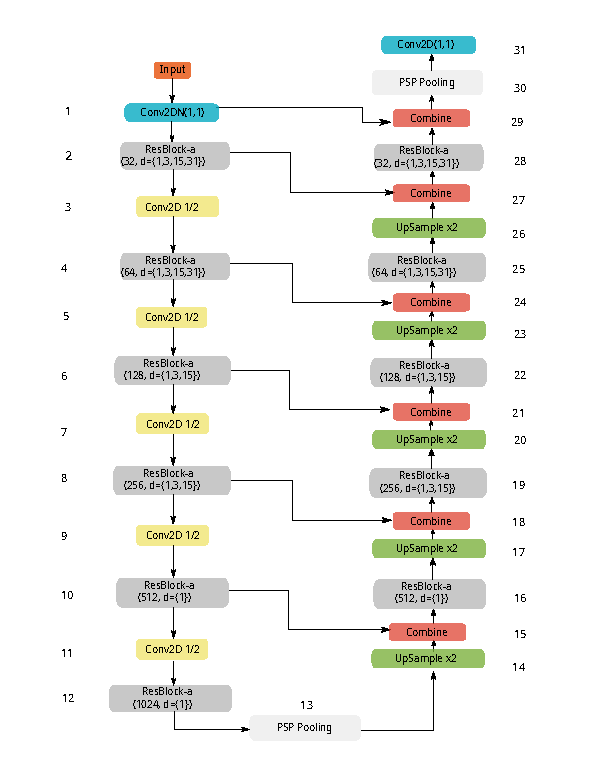
\includegraphics[width=0.7\textwidth,keepaspectratio]{Figures/resuneta_overview.pdf}
\caption[Obecný přehled architektury ResUNet-a]{Obecný přehled architektury ResUNet-a bez použití multi-taskového učení. Převzato z \cite{resuneta}. }
\label{fig:resuneta_overview}
\end{figure}

\textbf{Multi-taskové učení} představeno v originální literatuře slouží ke zlepšení výsledků segmentační úlohy. Při aplikaci multi-taskového učení se nahradí finální $1\times1$ konvoluční vrstva, PSP pooling vrstva a kombinační vrstva na výstupu jednodušší sítě ResUNet-a. Pro segmentační úlohu jsou si všechny 4 části na sobě komplementární a na sobě nezávisle vygenerovány. Je nutno podotknout, že tyto části nejsou určeny jako přímá součást finálních inferenčních výsledků, avšak pro vylepšení generalizační a sémanticky chápající schopnosti sítě během tréninku. Učením těchto doplňkových úloh získává síť další informace, které nepřímo přispívají ke zlepšení přesnosti a kvality primární úlohy: segmentace. Konkrétně se jedná o následující 4 části \cite{resuneta}: 
\begin{enumerate}
    \item Segmentační masky
    \item Hranové masky, pro zlepšení pochopení rozsahu segmentační úlohy
    \item Vzdálenostní masky, zlepšující \enquote{propojení} topologického uspořádání mezi třídami na obrazu, jako je např. mezi autem a cestou na které stojí. V orig. lit. zmíněná např. segmentační maska pro cestu s \enquote{dírou} v místě, kde má být auto. Oba tyto objekty zároveň panují jako vlastní třídy součástí sítě.
    \item Výstupu obrázku v barevném modelu HSV
\end{enumerate}
\endinput